\chapter{Density Matrix and Entropy for Networks}\label{C_Density_Matrix}

In many complex system one element can be influenced by another ones with which is not directing interacting. For example, considering the city mobility, the road forms the network, closing one road may create traffic in another roads that do not intersect the closed one. To study the correlation between the nodes of a network the communicability matrix was introduced \cite{Estrada_2008}.
We call it communicability because correlation as a different meaning in social science, they called in this way the interactions.

Interestingly, this matrix behave as quantum density matrix. Thus, it is a possible candidate to the role of network density matrix and, as a consequence, we can borrow some information quantities as entropy that were introduces for quantum many body and quantum computing, opening a connection between the network theory and quantum realm.

\section{Estrada's Communicability matrix}

Most of the study on complex networks focuses on the spread of information following the shorter path, namely the shortest sequence of links that connects two different nodes. 
However, this is not the only way the information can flow, there are plenty of other more long route that are also available, and this vision ignores completely the complexity of the network.
To overcome that we introduce the communicability matrix, defined to consider also these possible path to go beyond the shortest one \cite{Estrada_2012}. It consider the influence over all the path that cross the choose node, weighted by their length.
%This concept is similar to the correlation in physics: it indicates how a node is changes in response to a perturbation in another node. 

Let $G=(V,E)$ be an undirected graph composed of $N$ nodes and $E$ links and let $A$ be the adjacency matrix of the graph.
We can define the communicability matrix as
\begin{equation}
    G(A) = \sum_{k=1}^{\infty}c_k A^k
\end{equation}
and the communicability from node $i$ to node $j$ is given by $G_{ij}$. The power of the adjacency matrix $(A^k)_{ij}$ give us the number of path of length $k$ starting from node $i$ ending in node $j$.
The coefficients $c_k$ indicates the weight of the paths and it is heavier the longer is the path, this is made to give more relevance to the short ones respect to the long ones. It must be chosen such that the series is convergent, they also must penalize long paths to reflect the preference to the shorter one.

An intuitive choice is $c_k = \frac{1}{k!}$, which transforms the communicability into an exponential function \cite{Estrada_2008}
\begin{equation}\label{G_E}
    G^E(A) =\sum_{k=1}^{\infty} \frac{A^k}{k!} = e^{A} .
\end{equation}
We can generalize it adding a constant term $\beta$
\begin{equation}
    G^E(A) =\sum_{k=1}^{\infty} \frac{\beta A^k}{k!} = e^{\beta A} ,
\end{equation}
this formulation is similar to the thermal green function for quantum system with Hamiltonian $A$ and temperature $T = \frac{1}{\beta}$.

Alternatively, we can choose $c_k = \alpha^{k}$ with $\alpha<\frac{1}{\lambda_N}$, where $\lambda_N$ is the largest eigenvalue of the adjacency matrix \cite{Katz}. In this case, it becomes a geometrical series yielding
\begin{equation}\label{G_R}
    G^R(A) =\sum_{k=1}^{\infty} \alpha^k A^k = (I -\alpha A)^{-1}.
\end{equation}
The two formulations for the communicability matrix lead to the same result and conclusion for the network in the limit $\alpha \rightarrow \frac{1}{\lambda_N}$ and $\lambda_N -\lambda_{N-1}$ large \cite{Benzi_Klymko}.


From this, we can introduce an global index for the network that consider all the different possible communication as
\begin{equation}
    EE(A)  = \Tr\left[e^{\beta A}\right].
\end{equation}
In the literature it is called Estrada index \cite{Estrada_2008} and can be interpreted as the sum of all the self-communication, that is the sum of the paths that end in the same node they have started.

However, the communicability matrices \eqref{G_E} and \eqref{G_R} study only the network's topology, namely the paths, and ignore the presence of dynamics over the network that may change the way information spreads.

If we consider the simplest dynamics, the random walk, it is governed by the Laplacian matrix $L$. 
Thus, the communicability matrices for random walk are \cite{Estrada_2012}
\begin{equation}\label{Estrada indeces}
    \begin{split}
        G^E(L) &=\sum_{k=1}^{\infty} \frac{\beta^k L^k}{k!} = e^{\beta L}  \\ 
        G^R(L) &= \sum_{k=1}^{\infty} \alpha^k L^k \rightarrow \alpha^{-1} \tilde{L}^{-1}
    \end{split}
\end{equation}

where $\tilde{L}^{-1} = \sum_{i=2}^N \frac{1}{\mu}v_i^Tv_i$ is the Moore-Penrose generalized inverse of the Laplacian. Here, $\mu$ are the eigenvalue ordered from the smaller to the bigger such that $\mu_1 < \mu_2 < ... < \mu_N$, and $v_i$ the respective eigenvectors of the Laplacian matrix \cite{Generalized_inverse_Laplacian}.
Also, the Laplacian Estrada index is define as
\begin{equation}\label{EE_L}
    EE(L) = \Tr\left[e^{\beta L}\right].
\end{equation}

%While the previous quantities using the adjacency matrix focalized over the topological aspects of the network and information spread, the laplacian communicability matrix embodies also the dynamical ones since the laplacian is involved in the random walk over a network. 

\subsection{Hamiltonian formalism}
The formulae \eqref{Estrada indeces} can be motivated by studying a classic and quantum harmonic oscillator on a network.
Consider a set of $N$ harmonic oscillators with coupling matrix $K = A$, where $A$ is a symmetric adjacency matrix. In this way, the nodes are considered as particle of mass $m = 1$ connected by springs with constant $A_{ij}$. The network should not have self interacting nodes, thus $A_{ii} = 0$. The system is submerged in a thermal bath at the temperature $T$. We assume there are no dumping and no external forces acting in the system besides the thermal fluctuation. 
Let introduce a set of coordinates $q_i$ that indicates the displacement of the $i$ particle respect the equilibrium position, the elastic elastic potential can be define as
\begin{equation}
    V(q) = \frac{1}{4}\sum_{i\neq j} K_{ij}(q_i-q_j)^2 = \frac{1}{2}\sum_{j}K_{jj}q_j^2 - \frac{1}{2} \sum_{i\neq j}K_{ij}q_iq_j,
\end{equation}
where 
\begin{equation}
    K_{jj} = \sum_{j \neq i} K_{ij}.
\end{equation}

We set $H_{ij}= K_{jj}\delta_{ij} - K_{ij}$, therefore the potential can be written as
\begin{equation}
    V(q) = \frac{1}{2}\sum_{i,j} H_{ij} q_i q_j.
\end{equation}
The $H$ matrix is a laplacian matrix and it is equal to the Laplacian of the network $L = D - A$, where $D$ is the degree matrix. It holds the property $\sum_j H_{ij} = 0$, therefore it has not negative eigenvalues and one must be equal to zero.
The zero eigenvalue ensure us that the motion of the center of must is conserved. %% find a way to cite this sentence

We can write the Lagrangian of the system as
\begin{equation}
    \mathcal{L} = \frac{1}{2}\sum_{ij} \dot q_i G_{ij} \dot q_j - \frac{1}{2} \sum_{ij} q_iH_{ij}q_j.
\end{equation}

The equations of motion are
\begin{equation}
    \ddot q_i = -H_{ij} q_j.
\end{equation}

The eigenmodes of the system are defined by the solution of the equation 
\begin{equation}
    \omega^2 \phi_i = H_{ij} \phi_j.
\end{equation}

Rewriting it in matrices form
\begin{equation}
    |\Omega^2 - H| = |\Omega^2 - H|.
\end{equation}

Therefore, the spectral signature of the matrix $H = L$ are the same of the harmonic oscillator. In this way we can connect the harmonic oscillator and the master equation of a network and vice versa. Since $M$ is diagonal, $H$ and $L$ have the same support, eigenvectors and eigenvalues, leading to $E = \omega^2 = \lambda$, which creates a natural ranking between the eigenvectors. 

The Hamiltonian of the system is given by
\begin{equation}\label{H_L}
    H_L = \sum_i \frac{p_i^2}{2} + \sum_{ij} \frac{1}{2}L_{ij}q_iq_j.
\end{equation}

\subsection{Network of classic harmonic oscillators}

To combine this with the thermodynamics, let consider the presence of a thermal bath in the Hamiltonian formalism using the Langevin equation
\begin{equation}
    \begin{aligned}
        &\dot q_i = p_i; \\
        &\dot p_i  = -H_{ij}q_j - \gamma \sum_j \left(\delta_{ij} - 1_{ij}\right)p_j + \sqrt{2T\gamma}\xi_i(t),
    \end{aligned}
\end{equation}
where $\gamma$ is the friction coefficient, $T$ is the temperature (Boltzmann constant $K_B =1$), $\delta_{ij}$ the Kronecker delta and $1_{ij}$ the matrix with all entries equal to 1, $\xi_i(t)$ is white noise, namely
\begin{equation}\label{white_noise}
    \langle\xi_i(t)\rangle = 0 \qquad \langle\xi_i^2(t)\rangle = 1 
\end{equation}

The white noises must hold the condition $\sum_i \xi_i = 0$, that leaves invariant the motion of  system's center of mass but $\xi_i(t)$ are no more independent.
As a matter of fact, the derivative of $\sum_i p_i$ is zero, therefore it is an integral of motion,
\begin{equation}
    \frac{d}{dt} \sum_i \dot p_i = - \gamma \sum_{ij}\left(\delta_{ij} - 1_{ij}\right)p_j+ \cancel{\sqrt{2T\gamma}\sum_i\xi_i(t)} = 0.
\end{equation}

The condition over the white noises $\sum_i \xi_i = 0$ adds breaks the independence between them and it adds correlation.
We can rewriting the noise using i.i.d. white noise $w_i(t)$ as
\begin{equation}
    \xi_i(t) = w_i (t) + \frac{1}{N} \sum_k w_k(t).
\end{equation}
The covariance matrix of $\xi_i(t)$ can be written as
\begin{equation}
    \left<\xi_i(t)\xi_j(s)\right> = \left[\delta_{ij} - 1_{ij}\right]\delta(t-s)
\end{equation}

The distribution $\rho(q,p,t)$ is a Gaussian and satisfies the Fokker-Plank equation \cite{Fokker}
\begin{equation}
    \frac{\partial\rho}{\partial t} = -\sum_i p_i\frac{\partial \rho}{\partial q_i} + \sum_{ij} H_{ij}q_j\frac{\partial \rho}{\partial p_i} + \gamma\sum_{ij}\left(\delta_{ij}-1_{ij}\right)\left[\frac{\partial}{\partial p_i}p_j\rho + T \frac{\partial^2\rho}{\partial p_i \partial p_j}\right].
\end{equation}
The dynamics converges to a stationary distribution with time scale depending on the eigenvalue of the Laplacian matrix.  
The solution at equilibrium is
\begin{equation}
    \rho(q,p) = Z(\beta)^{-1} \exp\left[ -\beta \left( \sum_j {p_j^2} + \sum_{ij} \frac{1}{2}q_iH_{ij}q_j\right)\right],
\end{equation}
where $\beta = \frac{1}{T}$ and $Z(\beta)$ is the partition function defined as
\begin{equation}
    Z(\beta) = \int \prod_i dp_i dq_i \; \exp\left[ -\beta \left( \sum_j {p_j^2} + \sum_{ij} q_iH_{ij}q_j\right)\right].
\end{equation}

The marginal distribution on the coordinates is a Maxwell-Boltzmann distribution with the internal energy 
\begin{equation}
    \rho(q) = Z(\beta)^{-1} e^{-\beta \left(\sum_{ij} q_iH_{ij}q_j\right)}.
\end{equation}

If $H$ is symmetric, namely the detailed balance condition holds, we can diagonalize the equation obtaining the motion of independent oscillators in the same thermal bath.
Therefore, changing the basis from $q_i$ to $Q_\lambda$ eigenvectors of the Hamiltonian, the marginal distribution becomes
\begin{equation}\label{marginal_probability}
    \rho(q) = Z(\beta)^{-1} e^{-\beta \left(\sum_{\lambda \neq 0} Q_\lambda \lambda Q_\lambda\right)},
\end{equation}
with partition function 
\begin{equation}
    Z(\beta) = \int \prod_{\lambda\neq 0} dQ_\lambda e^{-\beta \left(\sum_{\lambda \neq 0} \lambda Q_\lambda^2\right)}.
\end{equation}

The thermal distribution does not involve the zero eigenmode since the thermal bath does not interact with it. Thus, we can project the system into a invariant subspace orthogonal to the stationary distribution. The oscillator modes $Q_\lambda$ remain the same of the unperturbed case. 
This is a consequence of the condition $\sum_i \xi_i = 0$.
%Moreover, this is also connected to the conservation of the stationary distribution of the master equation \eqref{stationary_distribution}. 
The distribution has mean $\left<Q_\lambda\right>= 0$ and the covariance matrix is diagonal with entries $\left<Q^2_\lambda\right>= \frac{1}{\beta \lambda}$.

The variance can be expresses as
\begin{equation}\label{classic_correlation}
    \mathrm{Cov}(Q) = \frac{1}{\beta}L^{-1},
\end{equation}
where ${L}^{-1} = \sum_{i=2}^N \frac{1}{\mu_i}v_i^Tv_i$ is the Moore-Penrose generalized inverse of the Laplacian. Here, $\mu$ are the eigenvalue ordered from the smaller to the bigger such that $\mu_1 < \mu_2 < ... < \mu_N$, and $v_i$ the respective eigenvectors of the Laplacian matrix \cite{Generalized_inverse_Laplacian}.

This is the same result as the Estrada's Communicability matrix $G^R(L)$ \eqref{Estrada indeces} with $\alpha=\beta$.
When $T\rightarrow 0$ the spread of information drops; and when $T\rightarrow +\infty$ it becomes instantaneous.

\subsection{Network of quantum harmonic oscillators}

Instead, for the quantum case ($\hbar = 1$), $H_L$, $q_i$ and $p_j$ are promoted to operators $\hat H_L$, $\hat q_i$ and $\hat p_j$ and  they satisfy the commutator relation $\left[\hat q_i, \hat p_j\right] = i \delta_{ij}$.

We need to add a new term; it should be considered as additional springs with constant $K'$ that connect each node to the ground: it prevent the the center of mass from moving. So the Hamiltonian becomes
\begin{equation}\label{H_L_QM}
    H_L = \sum_i\left(\frac{\hat p_i^2}{2}+\frac{K'}{2}\hat q_i^2\right) + \sum_{ij}\frac{1}{2} L_{ij}\hat q_i\hat q_j.
\end{equation}

We introduce the bosons creation and annihilation operators as
\begin{equation}
     \hat a_i = \frac{1}{\sqrt{2}}\left(\sqrt{\Omega} \hat q_i + \frac{i}{\sqrt{\Omega}}\hat p_i\right) \qquad 
     \hat a_i^\dagger = \frac{1}{\sqrt{2}}\left(\sqrt{\Omega} \hat q_i - \frac{i}{\sqrt{\Omega}}\hat p_i\right), 
\end{equation}
and the inverse as
\begin{equation}
    \hat q_i = \sqrt{\frac{1}{2\Omega}}\left(\hat a_i + \hat a_i^\dagger\right) \qquad
    \hat p_i = i\sqrt{\frac{\Omega}{2}}\left(\hat a_i - \hat a_i^\dagger\right),
\end{equation}
where $\Omega = \sqrt{K'}$.
They satisfy the commutation relation $\left[\hat a_i, \hat a^\dagger_j\right] = \delta_{ij}$. 

The Hamiltonian can be written as 
\begin{equation}
    \hat H_L = \sum_i \Omega \left(\hat a_i\hat a^\dagger_i + \frac{1}{2}\right) + \frac{1}{4\Omega}\sum_{ij}\left(\hat a_i +\hat a_i^\dagger\right)L_{ij}\left(\hat a_i +\hat a_i^\dagger\right).
\end{equation}

Since The network is undirected, $L$ is symmetric and, therefore, we can diagonalize it. The diagonalized laplacian is written in the form $\Lambda = OLO^T$.
This generates a new pair of bosons creation and annihilation operators respect the eigenvalue $\mu$ of the Laplacian
\begin{equation}
    b_\mu = \sum_j a_jO_{\mu j}  \qquad \hat b_\mu^\dagger = \sum_j a_j^\dagger O^T_{\mu j} .
\end{equation}

Thus, the new Hamiltonian becomes a sum of independent Hamiltonians
\begin{equation}
    \hat H_L = \sum_\mu \hat H_\mu,
\end{equation}
with
\begin{equation}
    \begin{split}
        \hat H_\mu &= \Omega \left(\hat b_\mu\hat b^\dagger_\mu + \frac{1}{2}\right) + \frac{1}{4\Omega}\mu\left(\hat b_\mu +\hat b_\mu^\dagger\right)^2\\
        &= \Omega \left(\hat b_\mu\hat b^\dagger_\mu + \frac{1}{2}\right) + \frac{1}{4\Omega}\mu\left[\left(\hat b_\mu\right)^2 +\left(\hat b_\mu^\dagger\right)^2 + 2 \hat b_\mu \hat b_\mu^\dagger + 1 \right]\\
        &= \Omega \left[ 1 + \frac{1}{2\Omega}\mu\right] \left(\hat b_\mu\hat b^\dagger_\mu + \frac{1}{2}\right) + \frac{1}{4\Omega}\mu\left[\left(\hat b_\mu\right)^2 +\left(\hat b_\mu^\dagger\right)^2 \right].
    \end{split}
\end{equation}

We now consider the system as fermionic so the modes do not excite beyond the first excitation state. In this way we can restrict the Hilbert state of a mode to the span of the ground state $\ket{g}$ and the first excited state $\ket{e_\mu}=b_\mu^\dagger\ket{g}$. A consequence of it is that the second term in the Hamiltonian cancel out. 


Now, we can compute the thermal Green function or Matsubara Green function for fermions $G$. This quantity describes the probability amplitude for the particle to travel from one state to the other in a given time $\tau$ (more detail in the Appendix \ref{Appendix_B}). For $\tau > 0$ it is

\begin{equation}
    \begin{split}
        G^L_{ij}(\beta, \tau > 0) &= \frac{\Tr\left[e^{-\beta \hat H_L}\hat a_i (\tau)  \hat a_j^\dagger\right]}{\Tr\left[e^{-\beta \hat H_L}\right]} \\
        &=\sum_{\mu\nu} O_{\mu i}\frac{\Tr\left[ (\tau) e^{-\beta \hat H_L} \hat b_\mu\hat b_\nu^\dagger\right]}{\Tr\left[e^{-\beta \hat H_L}\right]}O_{j\nu}\\
        &= \sum_{\mu} O_{i\mu}\left\{-e^{-\mu \tau}\left[\left(1-f\left( \Omega + \frac{1}{2\Omega^2}\mu\right)\right)\Theta(\tau)\right]\right\}O_{j\mu}\\
        &= \sum_{\mu} O_{i\mu}\left\{\frac{e^{-\mu \tau}}{e^{-\beta\left[ \Omega + \frac{1}{2\Omega^2}\mu\right]} + 1}\right\}O_{j\mu}\\
    \end{split}
\end{equation}
In the limit $\tau \rightarrow 0^+$ and $\beta$ large enough it tend to
\begin{equation}
    G^L(\beta) = \sum_{\mu} O_{i\mu}{e^{\beta\left[ \Omega + \frac{1}{2\Omega^2}\mu\right]}} O_{\mu i},
\end{equation}
that can be written as
\begin{equation}
    G^L_{ij}(\beta)= e^{\beta \Omega}e^{\frac{\beta \omega^2}{2\Omega}L}.
\end{equation}

Comparing it with the eq. \eqref{Estrada indeces}, choosing $2\Omega =\omega^2$ the two equations are related as
\begin{equation}
    G^R(L) = e^{-\beta\Omega}G^L(\beta).
\end{equation}
When the temperature $T \rightarrow 0$ the communicability between the nodes drops to zero and the perturbation does not spread across the network. Instead, when $T \rightarrow \infty$ the communicability tend to infinity and the perturbation spread instantaneously.  


\section{Density matrix and entropy for complex network}
%as in paper 2023 with the special case in paper 2020
The communicability matrix defined above possesses peculiar properties that make it suitable for use as a density matrix. Moreover, the presence of the Laplacian matrix ensure that it does not only consider the topological features of the network but also the dynamics. Taking the exponential communicability matrix as a reference, we can define a density matrix as
\begin{equation}\label{density_matrix}
    \hat \rho(\beta) = \frac{1}{Z} e^{-\beta \hat L} \qquad \mathrm{with} \qquad Z(\beta) = \Tr[e^{-\beta \hat L}],
\end{equation}
where $Z$ is the partition function and it is equal to the Laplacian Estrada index of the network \eqref{EE_L}.
It is a hermitian and positive defined matrix with trace equal to unity. 
It can be seen that $e^{-\beta L}$ is the propagator for diffusion equation in a network at time $t = \beta$.

From this, we can define the network's entropy as the Von Neumann entropy
\begin{equation} \label{entropy}
    S(\hat\rho) = -\Tr[\hat \rho \ln \hat \rho].
\end{equation}

Considering \eqref{density_matrix}, the network's entropy can be written also in the form
\begin{equation}\label{alternative_entropy}
    S(\hat\rho) = \beta \Tr\left[L\hat\rho\right] + \ln Z.
\end{equation}

The entropy is not negative and it is equal to zero if and only if the $\hat\rho$ is a pure state. It has a higher bound $S \leq \ln(N)$,  \cite{Nielsen_Chuang_2010}.

The entropy satisfy the sub-additivity property \cite{De_Domenico_2016}:
Let $\hat\rho$, $\hat\tau$ and $\hat\sigma$ be density matrices corresponding to the networks $G$, $H$, $I$ respectively. The networks $t$ and $S$ are subgraph of the network $G$ such that $G = H + I$.
If the sub-additivity is satisfied  then $S(\hat\rho) \leq S(\hat\tau) + S(\hat\sigma)$, the equivalence is obtain if the two subgraphs does not have nodes from the same component of $G$. In appendix \ref{C_sub_additivity} there is a mathematical proof.




Figure \ref{fig:ER-BA-WS} shows the entropy \eqref{entropy} for different types of networks\footnote{The python scripts can be found in the GitHub page of the author at the link: \url{https://github.com/ShqemzaMatteo/Master_thesis}}: a ring graph, an Erd\H{o}s-Rényi (E-R) random graph, a Barab\'asi-Albert (B-A) scale-free graph, and a Watts-Strogatz (W-S) small-sworld graph.

\begin{figure}[ht!]
    \centering
    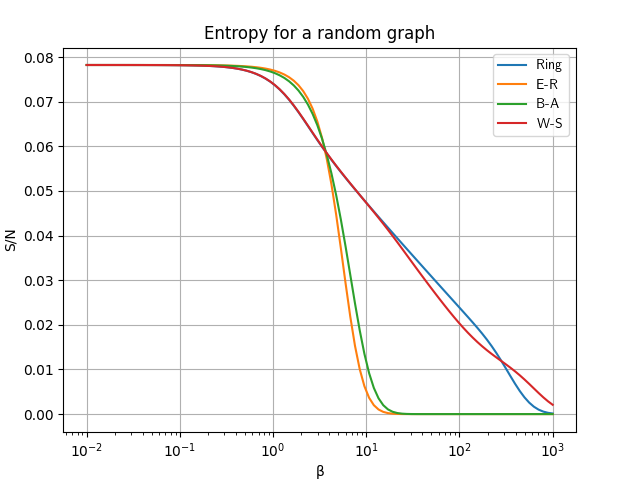
\includegraphics[width=0.75\linewidth]{image/random_graph.png}
    \caption{Plot of the network's entropy per node as a function of $\beta$ for different network types with $50$ nodes: a ring graph (blue), a Erd\H{o}s-Rényi (E-R) random graph with connectivity probability $0.7$ (orange), a Barab\'asi-Albert (B-A) scale-free graph with parameter $m=3$ (green), and a Watts-Strogatz (W-S) small world graph with parameter $K=3$ and rewire probability 0.2 (red). The x-axis has a logarithmic scale. For large $\beta$ the entropy tends to zero far all the networks.}
    \label{fig:ER-BA-WS}
\end{figure}

Using the density matrix, we can introduce also other thermodynamics quantities like the Helmoltz free energy $F = -\frac{1}{\beta} \ln Z$.


A possible interpretation of this density matrix is given by De Domenico \cite{De_Domenico_2020}.
Consider a network composed of $N$ nodes, encoded in the adjacency matrix $A$. Each node can be associated with a  value $n_i$ representing a property of the network, like the number of particles in the node in a diffusion model. 
The evolution of these variables is governed by the control operator $\hat L$. 

The network can be described using the Dirac notation. Let be $\ket{\psi} = \sum_i n_i \ket{i}$ the state of the system, where $\ket{i}$ is the canonical vector identifying the node $i$. The set $\{\ket{i}\}_{i=0}^N$ forms an orthogonal basis, satisfying $\braket{i}{j} = \delta_{ij}$, where $\delta_{ij}$ is the Kronecker delta.

The dynamics can be written as
\begin{equation} \label{time_evolution}
    \partial_t \ket{\psi(t)} = - \hat L \ket{\psi(t)},
\end{equation}
with the solution
\begin{equation}
    \ket{\psi(t)} = \hat G(t,0) \ket{\psi(0)}
\end{equation}
where $\hat G(t,0) = e^{-t\hat L}$ is the propagator and $\ket{\psi(0)}$ is the initial state. 

Since $\hat L$ is Hermitian, the propagator can be diagonalized in the orthogonal basis $\{\ket{v_\lambda}\}_\lambda$ of eigenvectors of the control operator
\begin{equation}\label{diagonal_propagator}
    \hat G(t,0) = \sum_\lambda e^{-t\lambda} \ket{v_\lambda}\bra{v_\lambda} = \sum_\lambda e^{-t\lambda} \hat \sigma_\lambda,
\end{equation}
where $\hat \sigma_\lambda$ is the projection over the left and right eigenvectors with the $\lambda$ eigenvalue. The operators do not depend on time, they are constant along the process, only the eigenvalues change.

The system relaxes to a stationary state $\ket{\psi_0}$ corresponding to the zero eigenvector.
We consider the system in the initial state $\ket{\psi} = \ket{\psi_0} + \ket{\Delta\psi}$, where $\ket{\Delta\psi}$ is a small perturbation relative to the stationary state. The initial perturbation can be decomposed as $\ket{\Delta\psi_0} = \sum_i \Delta_i \ket{i}$.
The time evolution of the state becomes
\begin{equation}
    \ket{\psi(t)} = G(t,0) \ket{\psi(0)} = \ket{\psi_0} + G(t,0)\ket{\Delta\psi} = \ket{\psi_0} + \ket{\Delta\psi(t)}
\end{equation}
with $\ket{\Delta\psi(t)} = e^{-t\hat L} \ket{\Delta \psi}$.

Since the stationary component is constant in time, we focus on the perturbation. 
The value of the perturbation at node $j$ at time $t$ is
\begin{equation}
    \braket{j}{\Delta\psi(t)} = \bra{j} e^{-t\hat L} \ket{\Delta\psi} =\sum_\lambda \bra{j} e^{-t\lambda} \hat \sigma_\lambda\ket{\Delta\psi} = \sum_i  \sum_\lambda \Delta_i e^{-t\lambda} \bra{j}  \hat \sigma_\lambda \ket{i}.
\end{equation}
We have used equation \eqref{diagonal_propagator} and the definition of the perturbation.
This equation shows that the perturbation travels through $N$ different streams, one for each $\sigma_\lambda$, with the stream's size $\Delta_i e^{-t\lambda}$. If $\Delta_i e^{-t\lambda} > 0$ the stream is active; if $\Delta_i e^{-t\lambda} = 0$ it is inactive. Negative stream coefficients imply an inverted flux from $j$ to $i$.
Sometimes, the dynamics traps part of the perturbation in a specific node. The trapped perturbation's size can be compute as
\begin{equation}
    T = \sum_i  \sum_\lambda \Delta_i e^{-t\lambda} \bra{i}  \hat \sigma_\lambda \ket{i} 
\end{equation} 

Assuming maximal uncertainty in the perturbation, obtainable when $\Delta_i = \Delta$, the equation reduces to
\begin{equation}
    T = \Delta \sum_i e^{-t\lambda} \bra{i}  \hat \sigma_\lambda \ket{i} = \Delta \Tr [\hat G(t,0)]
\end{equation}

Since the trapped perturbation regulates the stream's sizes, it can be responsible for the generation of the streams itself. 
Thus, we can define a density matrix 
\begin{equation}
    \hat \rho_t = \frac{1}{T} \Delta e^{-t\hat L} =  \frac{1}{Z} e^{-t\hat L},
\end{equation}
where $Z = \Tr[e^{-t\hat L}] $ is the partition function.
This density matrix can be interpreted as the probability that the perturbation will flow through a specific stream $\hat \sigma_l$ in the ensemble of all the possible streams \cite{De_Domenico_2020}.

The complexity of information streams can be quantified by the Von Neumann entropy.
When the information dynamics is described by a single information stream, a pure state, entropy is zero.
In contrast, as the information dynamics becomes more complex and diverse, the number of information streams increases, resulting in higher entropy.

\subsection{Kullback-Liebler and Jensen-Shannon Divergences}
Starting from the concept of entropy, we can also introduce the Kullback-Liebler (KL) divergence or relative entropy \cite{K-L_divergence} as
\begin{equation}\label{KL_divergence}
    D_{KL}(\hat \rho || \hat \sigma) = \Tr \left[\hat \rho \ln\left(\frac{\hat\sigma}{\hat\rho}\right)\right].
\end{equation}
It measure the close is the distribution $\hat \sigma$ to reproduce a event with real distribution $\hat \rho$. 
The KL divergence is always non negative and it equals zero when $\hat \rho = \hat \sigma$. It is not symmetric an unbounded \cite{J-S_divergence}.

It can be used to make comparisons between networks. Moreover, this concept we can be applied to the reconstruction of network starting from real data using the maximum likelihood estimation: it is to find the best model that reproduce the experimental data. In fact, the maximum likelihood estimation can be apply minimizing the Kullback-Liebler divergence between chosen network models and the dataset \cite{De_Domenico_2016}. This opens the door to the application of machine learning technique in complex network.


However the Kullback-Liebler divergence is not symmetric, therefore it can not be use as a metric. 
But we can symmetrize introducing the Jensen-Shannon (JS) divergence \cite{J-S_divergence} as
\begin{equation}\label{JS_metric}
    \mathcal{D}_{JS}(\hat\rho||\hat\sigma) =  \frac{1}{2}D(\hat \rho || \hat \mu) + \frac{1}{2}D(\hat \sigma || \hat \mu) = S(\hat\mu)-\frac{1}{2}\left[S(\hat\rho) + S(\hat\sigma)\right],
\end{equation}
where $\hat\mu =\frac{1}{2}(\hat\rho+\hat\sigma)$. 
\begin{figure}[ht!]
    \centering
    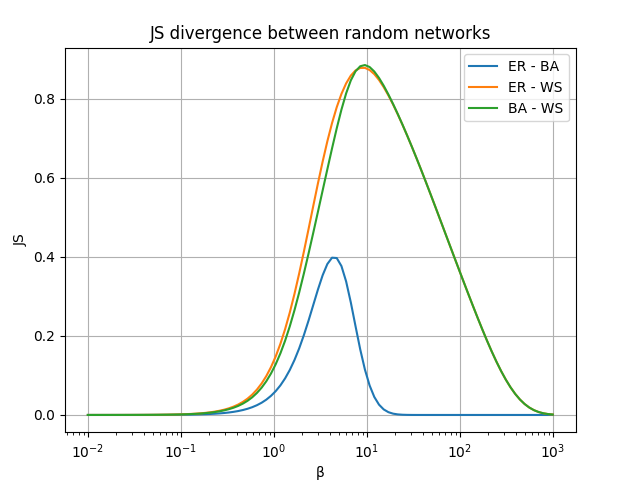
\includegraphics[width=0.75\textwidth]{image/JS_divergence.png}
    \caption{Plot of the KL divergence as a function of $\beta$ between different network types with $50$ nodes: a Erd\H{o}s-Rényi (E-R) random graph with connectivity probability $0.7$ and a Barab\'asi-Albert (B-A) scale-free graph with parameter $m=3$ (blue); a Erd\H{o}s-Rényi (E-R) random graph with connectivity probability $0.7$ and Watts-Strogatz (W-S) small world graph with parameter $K=3$ and rewire probability 0.2 (orange); a Barab\'asi-Albert (B-A) scale-free graph with parameter $m=3$ and a Watts-Strogatz (W-S) small world graph with parameter $K=3$ and rewire probability 0.2 (green). The x-axis has a logarithmic scale.The ER and BA networks are closer respect to a WS network. The divergence is maximum around $\beta = 10$.}
    \label{Fig:JS_divergence}
\end{figure}

The JS divergence is a bounded function \cite{J-S_divergence}
\begin{equation}
    0 \geq \mathcal{D}_{JS}(\hat\rho||\hat\sigma) \geq 1.
\end{equation}
$\left(\mathcal{D}_{JS}\right)^{\frac{1}{2}}$ defines a metric: it is symmetric, positive define, and hold the triangular inequality \cite{Jensen-Shannon_divergence}. 

%It has been use successfully to measure the distance between the layer of a multilayer network in order to aggregate them and eliminate the redundant layers \cite{multilayer}.
It has been use successfully to measure the distance between the network in order to aggregate them \cite{multilayer}.

Figure \ref{Fig:JS_divergence} shows the Jensen-Shannon divergence between an Erd\H{o}s-Rényi (E-R) random graph, a Barab\'asi-Albert (B-A) scale-free graph and a Watts-Strogatz (W-S) small-sworld graph \footnote{The python scripts can be found in the GitHub page of the author at the link: \url{https://github.com/ShqemzaMatteo/Master_thesis}}.